% 6. Descripción de la Competencia; 6.1. Estructura del Torneo; 12.1. Para Othello.
\section{Competencia de IAs en Othello}
\textit{Guía: 6. Descripción de la Competencia; 6.1. Estructura del Torneo; 12.1. Para Othello.}
\subsection{Agentes y metodología}
Se enfrentan \texttt{fija} y \texttt{etapas} con la misma búsqueda Alpha-Beta. El plan acordado comprende 13 aperturas de ocho colocaciones, dos asignaciones de color y profundidades 4, 5, 6 y 7: 104 partidas. Las aperturas se generan eligiendo acciones legales con semilla 20261008, rechazando equivalencias por simetría. Los desempates de búsqueda son deterministas; se exploran primero esquinas y luego coordenadas. Puntuación: victoria 1, empate 0.5, derrota 0. Ambos rivales usan la misma profundidad en cada partida.

Por decisión del usuario, la ejecución se limita al piloto de una apertura, con ocho partidas; las 96 restantes quedan pendientes. El hardware, versiones y huellas de código están en el manifiesto del experimento. Los tiempos miden búsqueda e instrumentación, excluyen apertura, red, dibujo y escritura. Un nodo evaluado es una hoja terminal o una hoja de corte, no todo nodo visitado. Se conserva un registro por movimiento y evaluaciones intermedias desde negras.

\subsection{Resultados y discusión}
% 12.1. Para Othello; 16. Formato de Tablas y Figuras. Generado por analizar.py.
\begin{table}[htbp]
\centering\small
\caption{Othello: resultados internos disponibles a igual profundidad. V/D/E: victorias/derrotas/empates; puntos: 1/0/0.5.}
\label{tab:othello_resultados}
\begin{tabular}{lrrrrrrr}
\toprule
Agente & Prof. & V & D & E & $\overline{\Delta}$ & Puntos & s/jugada \\
\midrule
etapas & 4 & 1 & 1 & 0 & 0.00 & 1.0 & 0.268 \\
fija & 4 & 1 & 1 & 0 & 0.00 & 1.0 & 0.276 \\
etapas & 5 & 0 & 2 & 0 & -25.00 & 0.0 & 0.835 \\
fija & 5 & 2 & 0 & 0 & 25.00 & 2.0 & 0.755 \\
etapas & 6 & 0 & 2 & 0 & -19.00 & 0.0 & 4.564 \\
fija & 6 & 2 & 0 & 0 & 19.00 & 2.0 & 4.085 \\
etapas & 7 & 1 & 1 & 0 & -1.00 & 1.0 & 23.230 \\
fija & 7 & 1 & 1 & 0 & 1.00 & 1.0 & 23.124 \\
\bottomrule
\end{tabular}
\end{table}

% 12.1. Para Othello; 13. Métodos Estadísticos Requeridos. Generado por analizar.py.
Se completaron 8 de 104 partidas planificadas; quedan 96 pendientes. 
La versión etapas obtuvo 2 victorias, 6 derrotas y 0 empates. 
La versión fija obtuvo 6 victorias, 2 derrotas y 0 empates. 
Estos totales mezclan profundidades y sólo describen las partidas disponibles; no prueban superioridad general. 
A profundidad 4, con 1 bloque(s), el valor $p$ binomial bilateral es no aplicable (bloque empatado). 
A profundidad 5, con 1 bloque(s), el valor $p$ binomial bilateral es 1.000. 
A profundidad 6, con 1 bloque(s), el valor $p$ binomial bilateral es 1.000. 
A profundidad 7, con 1 bloque(s), el valor $p$ binomial bilateral es no aplicable (bloque empatado). 
El tamaño muestral limita la inferencia. Los intervalos y las condiciones de aplicabilidad se conservan en el registro estadístico reproducible.

\begin{figure}[htbp]
\centering
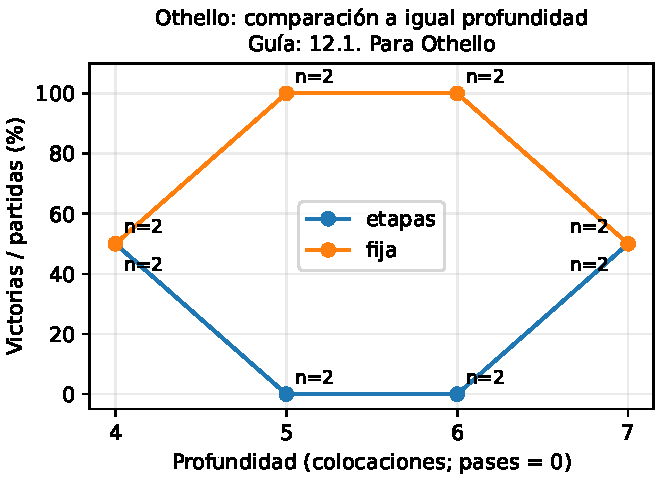
\includegraphics[width=.48\linewidth]{../datos/othello/analisis/victorias_profundidad_othello.pdf}
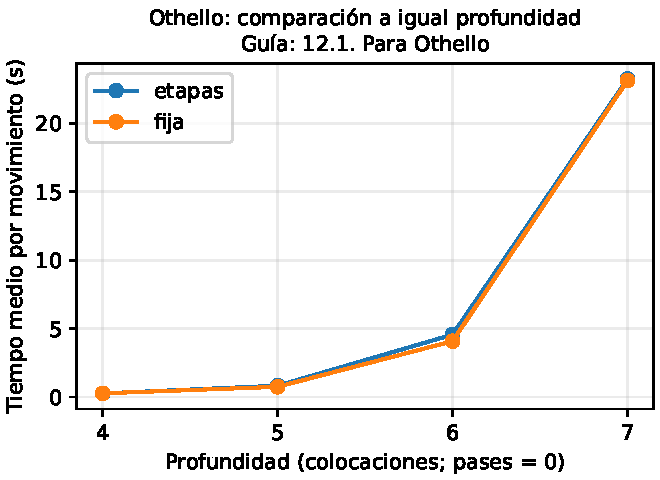
\includegraphics[width=.48\linewidth]{../datos/othello/analisis/tiempo_profundidad_othello.pdf}
\caption{Piloto interno: victorias y tiempo medio por movimiento frente a profundidad. Cada nivel usa ambos colores de una apertura; no son réplicas independientes.}
\label{fig:othello_profundidad}
\end{figure}
El cliente automático permite conectarse al servidor del docente, y el torneo acepta adaptadores de otros grupos. No se recibieron agentes externos; su competencia está pendiente y no se sustituye por estos enfrentamientos internos.
